\section{Naravna in cela števila}

\begin{frame}
    \sectionpage
\end{frame}

\begin{frame}
    \tableofcontents[currentsection, hideothersubsections]
\end{frame}
        
    \subsection{Naravna števila}

        \begin{frame}
            \frametitle{Naravna števila}

                \only<2->{\begin{alertblock}{Množica naravnih števil}
                    \only<3->{\textbf{Naravna števila} so števila s katerimi štejemo.}
                    \only<4->{$$\mathbf{\mathbb{N}=\{1, 2, 3, 4, \ldots\}}$$}
                \end{alertblock}}

                \only<5->{\begin{block}{}
                    Množico naravnih števil definirajo \textbf{Peanovi aksiomi}:
                    \begin{enumerate}
                        \item<6-> Vsako naravno število $n$ ima svojega \textbf{naslednika} $n+1$.
                        \item<7-> Število $1$ je naravno število, ki ni naslednik nobenega naravnega števila.
                        \item<8-> Različni naravni števili imata različna naslednika: $n+1 \neq m+1; n \neq m$.
                        \item<9-> Če neka trditev velja z vsakim naravnim številom tudi za njegovega naslednika, velja za vsa naravna števila. (\textit{aksiom/princip popolne indukcije})
                    \end{enumerate}

                \end{block}}
        \end{frame}

        \begin{frame}

            \only<2->{\begin{block}{}
                Naravna števila uredimo po velikosti in predstavimo s \textbf{točko} na \textbf{številski premici}.
                \only<3->{\begin{figure}
                    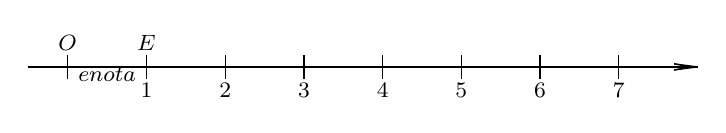
\begin{tikzpicture}
                        % \clip (0,0) rectangle (14.000000,10.000000);
                        {\footnotesize
                        
                        % Drawing segment a b
                        \draw [line width=0.016cm] (0.500000,0.500000) -- (9.000000,0.500000);%
                        
                        % Drawing arrow a b 1.00
                        \draw [line width=0.016cm] (8.702567,0.539158) -- (9.000000,0.500000);%
                        \draw [line width=0.016cm] (8.702567,0.539158) -- (8.900856,0.500000);%
                        \draw [line width=0.016cm] (8.702567,0.460842) -- (9.000000,0.500000);%
                        \draw [line width=0.016cm] (8.702567,0.460842) -- (8.900856,0.500000);%
                        
                        % Drawing segment c d
                        \draw [line width=0.016cm] (1.000000,0.350000) -- (1.000000,0.650000);%
                        
                        % Drawing segment e f
                        \draw [line width=0.016cm] (2.000000,0.350000) -- (2.000000,0.650000);%
                        
                        % Drawing segment g h
                        \draw [line width=0.016cm] (3.000000,0.350000) -- (3.000000,0.650000);%
                        
                        % Drawing segment i j
                        \draw [line width=0.016cm] (4.000000,0.350000) -- (4.000000,0.650000);%
                        
                        % Drawing segment k l
                        \draw [line width=0.016cm] (5.000000,0.350000) -- (5.000000,0.650000);%
                        
                        % Drawing segment m n
                        \draw [line width=0.016cm] (6.000000,0.350000) -- (6.000000,0.650000);%
                        
                        % Drawing segment o p
                        \draw [line width=0.016cm] (7.000000,0.350000) -- (7.000000,0.650000);%
                        
                        % Drawing segment r s
                        \draw [line width=0.016cm] (8.000000,0.350000) -- (8.000000,0.650000);%
                        
                        % Marking point O
                        \draw (1.000000,0.600000) node [anchor=south] { $O$ };%
                        
                        % Marking point E
                        \draw (2.000000,0.600000) node [anchor=south] { $E$ };%
                        
                        % Marking point 1
                        \draw (2.000000,0.400000) node [anchor=north] { $1$ };%
                        
                        % Marking point 2
                        \draw (3.000000,0.400000) node [anchor=north] { $2$ };%
                        
                        % Marking point 3
                        \draw (4.000000,0.400000) node [anchor=north] { $3$ };%
                        
                        % Marking point 4
                        \draw (5.000000,0.400000) node [anchor=north] { $4$ };%
                        
                        % Marking point 5
                        \draw (6.000000,0.400000) node [anchor=north] { $5$ };%
                        
                        % Marking point 6
                        \draw (7.000000,0.400000) node [anchor=north] { $6$ };%
                        
                        % Marking point 7
                        \draw (8.000000,0.400000) node [anchor=north] { $7$ };%
                        
                        % Marking point {enota}
                        \draw (1.500000,0.600000) node [anchor=north] { ${enota}$ };%
                        }
                    \end{tikzpicture}
                        
                \end{figure}}

            \end{block}}

            \only<4->{\begin{block}{}
                Vsako število zapišemo s \textbf{številko}. 
                Za zapis številke uporabljamo \textbf{števke}. Te so $0, 1, 2, 3, 4, 5, 6, 7, 8, 9$.
            \end{block}}

            \only<5->{\begin{block}{}
                Posamezne števke večmestnega števila od desne proti levi predstavljajo: \textbf{enice}, \textbf{desetice}, \textbf{stotice}, \textbf{tisočice}, ...
            \end{block}}

            \only<6->{\begin{block}{}
                Število, ki je zapisano s črkovnimi oznakami števk označimo s črto nad zapsiom črkovne oznake.
                \only<7->{$$ \overline{xy}=10x+y \quad \quad \quad \overline{xyz}=100x+10y+z$$}
            \end{block}}

            
        \end{frame}

        \begin{frame}
            \frametitle{Operacije v množici $\mathbb{N}$}

            \only<2->{\begin{alertblock}{Seštevanje}
                \only<3->{Poljubnima naravnima številoma $x$ in $y$ priredimo \textbf{vsoto} $\mathbf{x+y}$.}
            \end{alertblock}}

            \only<4->{\begin{block}{}
                Število $x$ oziroma $y$ imenujemo \textbf{seštevanec} ali \textbf{sumand} ali \textbf{člen}. 

                \only<5->{Število $x+y$ pa imenujemo \textbf{vsota} ali \textbf{summa}. }

            \only<6->{\begin{figure}
                \begin{tikzpicture}
                    % \clip (0,0) rectangle (14.000000,10.000000);
                    {\footnotesize
                    
                    % Drawing segment a b
                    \draw [line width=0.016cm] (5.000000,0.500000) -- (5.000000,2.500000);%
                    
                    % Drawing segment b d
                    \draw [line width=0.016cm] (5.000000,2.500000) -- (7.000000,2.500000);%
                    
                    % Drawing segment c d
                    \draw [line width=0.016cm] (7.000000,0.500000) -- (7.000000,2.500000);%
                    
                    % Drawing segment c a
                    \draw [line width=0.016cm] (7.000000,0.500000) -- (5.000000,0.500000);%
                    
                    % Drawing segment e f
                    \draw [line width=0.016cm] (7.000000,1.500000) -- (9.000000,1.500000);%
                    
                    % Drawing arrow e f 1.00
                    \draw [line width=0.016cm] (8.702567,1.539158) -- (9.000000,1.500000);%
                    \draw [line width=0.016cm] (8.702567,1.539158) -- (8.900856,1.500000);%
                    \draw [line width=0.016cm] (8.702567,1.460842) -- (9.000000,1.500000);%
                    \draw [line width=0.016cm] (8.702567,1.460842) -- (8.900856,1.500000);%
                    
                    % Drawing segment g h
                    \draw [line width=0.016cm] (2.500000,1.000000) -- (5.000000,1.000000);%
                    
                    % Drawing segment i j
                    \draw [line width=0.016cm] (2.500000,2.000000) -- (5.000000,2.000000);%
                    
                    % Drawing arrow g h 1.00
                    \draw [line width=0.016cm] (4.702567,1.039158) -- (5.000000,1.000000);%
                    \draw [line width=0.016cm] (4.702567,1.039158) -- (4.900856,1.000000);%
                    \draw [line width=0.016cm] (4.702567,0.960842) -- (5.000000,1.000000);%
                    \draw [line width=0.016cm] (4.702567,0.960842) -- (4.900856,1.000000);%
                    
                    % Drawing arrow i j 1.00
                    \draw [line width=0.016cm] (4.702567,2.039158) -- (5.000000,2.000000);%
                    \draw [line width=0.016cm] (4.702567,2.039158) -- (4.900856,2.000000);%
                    \draw [line width=0.016cm] (4.702567,1.960842) -- (5.000000,2.000000);%
                    \draw [line width=0.016cm] (4.702567,1.960842) -- (4.900856,2.000000);%
                    
                    % Marking point {vsota}
                    \draw (8.000000,1.500000) node [anchor=south] { ${vsota}$ };%
                    
                    % Marking point {summa}
                    \draw (8.000000,1.500000) node [anchor=north] { ${summa}$ };%
                    
                    % Marking point {se�tevanec}
                    \draw (3.750000,1.000000) node [anchor=south] { ${seštevanec}$ };%
                    
                    % Marking point {sumand}
                    \draw (3.750000,1.000000) node [anchor=north] { ${sumand}$ };%
                    
                    % Marking point {se�tevanec}
                    \draw (3.750000,2.000000) node [anchor=south] { ${seštevanec}$ };%
                    
                    % Marking point {sumand}
                    \draw (3.750000,2.000000) node [anchor=north] { ${sumand}$ };%
                    
                    % Drawing segment x y
                    \draw [line width=0.032cm] (6.000000,1.000000) -- (6.000000,2.000000);%
                    
                    % Drawing segment z w
                    \draw [line width=0.032cm] (5.500000,1.500000) -- (6.500000,1.500000);%
                    }
                    \end{tikzpicture}
                    
            \end{figure}}


            \end{block}}


            \only<7->{\begin{block}{}
                Vsota naravnih števil je naravno število: $x, y \in \mathbb{N} \Rightarrow x+y \in \mathbb{N}$.

            \end{block}}

        \end{frame}

        \begin{frame}
            \only<2->{\begin{alertblock}{Množenje}
                \only<3->{Poljubnima naravnima številoma $x$ in $y$ priredimo \textbf{produkt} $\mathbf{x\cdot y}$.}
            \end{alertblock}}

            \only<4->{\begin{block}{}
                Število $x$ oziroma $y$ imenujemo \textbf{množenec} ali \textbf{faktor}. 

                \only<5->{Število $x\cdot y$ pa imenujemo \textbf{zmnožek} ali \textbf{produkt}. }

                \only<6->{\begin{figure}
                \begin{tikzpicture}
                    % \clip (0,0) rectangle (14.000000,10.000000);
                    {\footnotesize
                    
                    % Drawing segment a b
                    \draw [line width=0.016cm] (5.000000,0.500000) -- (5.000000,2.500000);%
                    
                    % Drawing segment b d
                    \draw [line width=0.016cm] (5.000000,2.500000) -- (7.000000,2.500000);%
                    
                    % Drawing segment c d
                    \draw [line width=0.016cm] (7.000000,0.500000) -- (7.000000,2.500000);%
                    
                    % Drawing segment c a
                    \draw [line width=0.016cm] (7.000000,0.500000) -- (5.000000,0.500000);%
                    
                    % Drawing segment e f
                    \draw [line width=0.016cm] (7.000000,1.500000) -- (9.000000,1.500000);%
                    
                    % Drawing arrow e f 1.00
                    \draw [line width=0.016cm] (8.702567,1.539158) -- (9.000000,1.500000);%
                    \draw [line width=0.016cm] (8.702567,1.539158) -- (8.900856,1.500000);%
                    \draw [line width=0.016cm] (8.702567,1.460842) -- (9.000000,1.500000);%
                    \draw [line width=0.016cm] (8.702567,1.460842) -- (8.900856,1.500000);%
                    
                    % Drawing segment g h
                    \draw [line width=0.016cm] (2.500000,1.000000) -- (5.000000,1.000000);%
                    
                    % Drawing segment i j
                    \draw [line width=0.016cm] (2.500000,2.000000) -- (5.000000,2.000000);%
                    
                    % Drawing arrow g h 1.00
                    \draw [line width=0.016cm] (4.702567,1.039158) -- (5.000000,1.000000);%
                    \draw [line width=0.016cm] (4.702567,1.039158) -- (4.900856,1.000000);%
                    \draw [line width=0.016cm] (4.702567,0.960842) -- (5.000000,1.000000);%
                    \draw [line width=0.016cm] (4.702567,0.960842) -- (4.900856,1.000000);%
                    
                    % Drawing arrow i j 1.00
                    \draw [line width=0.016cm] (4.702567,2.039158) -- (5.000000,2.000000);%
                    \draw [line width=0.016cm] (4.702567,2.039158) -- (4.900856,2.000000);%
                    \draw [line width=0.016cm] (4.702567,1.960842) -- (5.000000,2.000000);%
                    \draw [line width=0.016cm] (4.702567,1.960842) -- (4.900856,2.000000);%
                    
                    % Marking point {zmno�ek}
                    \draw (8.000000,1.500000) node [anchor=south] { ${zmnožek}$ };%
                    
                    % Marking point {produkt}
                    \draw (8.000000,1.500000) node [anchor=north] { ${produkt}$ };%
                    
                    % Marking point {mno�enec}
                    \draw (3.750000,1.000000) node [anchor=south] { ${množenec}$ };%
                    
                    % Marking point {faktor}
                    \draw (3.750000,1.000000) node [anchor=north] { ${faktor}$ };%
                    
                    % Marking point {mno�enec}
                    \draw (3.750000,2.000000) node [anchor=south] { ${množenec}$ };%
                    
                    % Marking point {faktor}
                    \draw (3.750000,2.000000) node [anchor=north] { ${faktor}$ };%
                    
                    % Drawing circle k
                    \draw [line width=0.016cm] (6.000000,1.500000) circle (0.100000);%
                    
                    % Filling circle k
                    \fill (6.000000,1.500000) circle (0.100000);%
                    }
                    \end{tikzpicture}
                    
            \end{figure}}

            \end{block}}


            \only<7->{\begin{block}{}
                Produkt naravnih števil je naravno število: $x, y \in \mathbb{N} \Rightarrow x\cdot y \in \mathbb{N}$.
            \end{block}}

            \only<8->{\begin{block}{}
                Število $\mathbf{1}$ je \textbf{nevtralni element} za mmnoženje: $1\cdot x = x$.
            \end{block}}

        \end{frame}

        \begin{frame}
            

            \only<2->{\begin{alertblock}{Odštevanje}
                \only<3->{Številoma $x$ in $y$, pri čemer je $x$ večje od $y$ ($x>y$), priredimo \textbf{razliko} $\mathbf{x-y}$.}
            \end{alertblock}}

            \only<4->{\begin{block}{}
                Število $x$ imenujemo \textbf{zmanjševanec} ali \textbf{minuend}, število $y$  pa imenujemo \textbf{odštevanec} ali \textbf{subtrahend}. 

                \only<5->{Številu $x-y$ rečemo \textbf{razlika} ali \textbf{diferenca}. }

                \only<6->{\begin{figure}
                    \begin{tikzpicture}
                        % \clip (0,0) rectangle (14.000000,10.000000);
                        {\footnotesize
                        
                        % Drawing segment a b
                        \draw [line width=0.016cm] (5.000000,0.500000) -- (5.000000,2.500000);%
                        
                        % Drawing segment b d
                        \draw [line width=0.016cm] (5.000000,2.500000) -- (7.000000,2.500000);%
                        
                        % Drawing segment c d
                        \draw [line width=0.016cm] (7.000000,0.500000) -- (7.000000,2.500000);%
                        
                        % Drawing segment c a
                        \draw [line width=0.016cm] (7.000000,0.500000) -- (5.000000,0.500000);%
                        
                        % Drawing segment e f
                        \draw [line width=0.016cm] (7.000000,1.500000) -- (9.000000,1.500000);%
                        
                        % Drawing arrow e f 1.00
                        \draw [line width=0.016cm] (8.702567,1.539158) -- (9.000000,1.500000);%
                        \draw [line width=0.016cm] (8.702567,1.539158) -- (8.900856,1.500000);%
                        \draw [line width=0.016cm] (8.702567,1.460842) -- (9.000000,1.500000);%
                        \draw [line width=0.016cm] (8.702567,1.460842) -- (8.900856,1.500000);%
                        
                        % Drawing segment g h
                        \draw [line width=0.016cm] (2.500000,1.000000) -- (5.000000,1.000000);%
                        
                        % Drawing segment i j
                        \draw [line width=0.016cm] (2.500000,2.000000) -- (5.000000,2.000000);%
                        
                        % Drawing arrow g h 1.00
                        \draw [line width=0.016cm] (4.702567,1.039158) -- (5.000000,1.000000);%
                        \draw [line width=0.016cm] (4.702567,1.039158) -- (4.900856,1.000000);%
                        \draw [line width=0.016cm] (4.702567,0.960842) -- (5.000000,1.000000);%
                        \draw [line width=0.016cm] (4.702567,0.960842) -- (4.900856,1.000000);%
                        
                        % Drawing arrow i j 1.00
                        \draw [line width=0.016cm] (4.702567,2.039158) -- (5.000000,2.000000);%
                        \draw [line width=0.016cm] (4.702567,2.039158) -- (4.900856,2.000000);%
                        \draw [line width=0.016cm] (4.702567,1.960842) -- (5.000000,2.000000);%
                        \draw [line width=0.016cm] (4.702567,1.960842) -- (4.900856,2.000000);%
                        
                        % Marking point {razlika}
                        \draw (8.000000,1.500000) node [anchor=south] { ${razlika}$ };%
                        
                        % Marking point {diferenca}
                        \draw (8.000000,1.500000) node [anchor=north] { ${diferenca}$ };%
                        
                        % Marking point {od�tevanec}
                        \draw (3.750000,1.000000) node [anchor=south] { ${odštevanec}$ };%
                        
                        % Marking point {subtrahend}
                        \draw (3.750000,1.000000) node [anchor=north] { ${subtrahend}$ };%
                        
                        % Marking point {zmanj�evanec}
                        \draw (3.750000,2.000000) node [anchor=south] { ${zmanjševanec}$ };%
                        
                        % Marking point {minuend}
                        \draw (3.750000,2.000000) node [anchor=north] { ${minuend}$ };%
                        
                        % Drawing segment z w
                        \draw [line width=0.032cm] (5.500000,1.500000) -- (6.500000,1.500000);%
                        }
                        \end{tikzpicture}
                        
            \end{figure}}
        \end{block}}

            \only<7->{\begin{block}{}
                Razlika je število, ki ga moramo prišteti številu $y$, da dobimo število $x$.
                \only<8->{$$ (x-y)+y=x $$}
            \end{block}}

        \end{frame}

        \begin{frame}
            \only<2->{\begin{block}{}
                Seštevanje in množenje sta \textit{dvočleni notranji operaciji} v množici naravnih števil $\mathbb{N}$.

                \only<3->{Odštevanje pa ni notranja operacija v množici naravnih števil $\mathbb{N}$.}
            \end{block}}

            \only<4->{\begin{block}{Vrstni red operacij}
                \only<5->{Prednost pri računanju imajo \textbf{oklepaji} (najprej najbolj notranji),} 
                \only<6->{nato sledi \textbf{množenje},}
                \only<7->{na koncu pa imamo še \textbf{seštevanje} in \textbf{odštevanje}.}
            \end{block}}

            \only<8->{\begin{block}{}
                Kadar v izrazu nastopajo enakovredne računske operacije, računamo od leve proti desni.
            \end{block}}

            \only<9->{\begin{block}{}
                Pri množenju količin, ki so označene s črkovnimi oznakami, piko, ki označuje operacijo množenja ponavadi opustimo.
                \only<10->{$$ x\cdot y = xy$$}
            \end{block}}


        \end{frame}

        \begin{frame}
            \frametitle{Osnovni računski zakoni v $\mathbb{N}$}

            \only<2->{\begin{block}{Komutativnost seštevanja -- zakon o zamenjavi členov}
                \only<3->{$$ \mathbf{x+y=y+x}$$}
                \only<4->{Vsota ni odvisna od vrstnega reda seštevanja.}
            \end{block}}

            \only<5->{\begin{block}{Asociativnost seštevanja -- zakon o poljubnem združevanju členov}
                \only<6->{$$ \mathbf{(x+y)+z=x+(y+z)}$$}
                \only<7->{Vsota več kot dveh sumandov ni odvisna od združevanja po dveh sumandov.}
            \end{block}}

        \end{frame}

        \begin{frame}


            \only<2->{\begin{block}{Komutativnost množenja -- zakon o zamenjavi faktorjev}
                \only<3->{$$ \mathbf{x\cdot y=y\cdot x}$$}
                \only<4->{Produkt ni odvisen od vrstnega reda faktorjev.}
            \end{block}}

            \only<5->{\begin{block}{Asociativnost množenja -- zakon o poljubnem združevanju faktorjev}
                \only<6->{$$ \mathbf{(x\cdot y)\cdot z=x\cdot (y\cdot z)}$$}
                \only<7->{Produkt več kot dveh sumandov ni odvisen od združevanja faktorjev.}
            \end{block}}

            \only<8->{\begin{block}{Distributivnost -- zakon o razčlenjevanju}
                \only<9->{$$ \mathbf{x\cdot z+y\cdot z = (x+y)\cdot z} $$}
                \only<10->{Če to beremo iz desne proti levi, rečemu tudi \textit{pravilo izpostavljanja skupnega faktorja}.}
            \end{block}}

        \end{frame}

        \begin{frame}
            \only<2->{\begin{exampleblock}{Naloga}
                Izračunajte.
                \only<3->{\begin{itemize}
                    \item $(1+2\cdot 7)+3\cdot(2\cdot 2+7)$ \\ ~
                    \item $3\cdot(2+3\cdot 5)\cdot(2+1)$ \\ ~
                    \item $7+(2+6\cdot 3)+(8+4\cdot 5)$ \\ ~
                    \item $11\cdot 4+(12-6)\cdot 5$ \\ ~
                    \item $8+2\cdot(3+7)-15$ \\ ~
                    \item $37-5\cdot(10-3)$ \\ ~
                \end{itemize}}
            \end{exampleblock}}
        \end{frame}

        \begin{frame}
            \only<2->{\begin{exampleblock}{Naloga}
                Hitro izračunajte.
                \only<3->{\begin{itemize}
                    \item $45+37+15$ 
                    \item $108+46-28$
                    \item $5\cdot 13\cdot 8$
                    \item $4\cdot 7\cdot 25$
                    \item $(7+3)\cdot 2\cdot 5$
                    \item $15\cdot(4+6)\cdot 2$
                    \item $3\cdot 5+7\cdot 5$
                    \item $8\cdot 12+6\cdot 8$
                \end{itemize}}
            \end{exampleblock}}
        \end{frame}

        \begin{frame}
            \only<2->{\begin{exampleblock}{Naloga}
                Zapišite račun glede na besedilo in izračunajte.
                \only<3->{\begin{itemize}
                    \item Produktu števil $12$ in $27$ odštejte razliko števil $19$ in $11$. \\ ~
                    \item Vsoti produkta $4$ in $12$ ter produkta $5$ in $16$ odštejte $8$. \\ ~
                    \item Vsoto števil $42$ in $23$ pomnožite z razliko števil $58$ in $29$. \\ ~
                    \item Produkt števil $14$ in $17$ pomnožite z vsoto števil $5$ in $16$. \\ ~ \\ ~
                \end{itemize}}
            \end{exampleblock}}
        \end{frame}

        \begin{frame}
            \only<2->{\begin{exampleblock}{Naloga}
                Rešite besedilno nalogo.
                \only<3->{\begin{itemize}
                    \item V trgovini kupimo tri litre mleka in štiri čokoladne pudinge v prahu. Če stane liter mleka $95$ centov,
                        čokoladni puding v prahu pa $24$ centov, koliko moramo plačati? \\ ~ \\ ~ \\ ~ \\ ~
                    \item Manca bo kuhala rižoto za štiri otroke in šest odraslih. Za otroško porcijo rižote zadošča $45~g$ riža,
                        za odraslo pa $75~g$. Koliko riža mora dati kuhati za rižoto? \\ ~ \\ ~ \\ ~ \\ ~
                \end{itemize}}
            \end{exampleblock}}
        \end{frame}

\subsection{Cela števila}
        \begin{frame}
            \frametitle{Cela števila}

                \only<2->{\begin{alertblock}{Množica celih števil}
                    \only<3->{$$\mathbf{\mathbb{Z} = \{\ldots, -2, -1, 0, 1, 2, 3, \ldots\}}$$}
                \end{alertblock}}

                \only<4->{\begin{block}{}
                    Množica celih števil $\mathbb{Z}$ je definirana kot unija treh množic:
                        \begin{itemize}
                            \item<5-> množica \textbf{pozitivnih celih števil} ($\mathbb{Z}^+$) -- naravna števila $\mathbb{N}$;
                            \item<6-> \textbf{število 0};
                            \item<7-> množica \textbf{negativnih celih števil} ($\mathbb{Z}^-$) -- nasprotna števila vseh naravnih števil.
                        \end{itemize}
                      \only<8->{$$\mathbb{Z} = \mathbb{Z}^- \cup \{0\} \cup \mathbb{Z}^+$$}

                \end{block}}

                \only<9->{\begin{block}{}
                    \textbf{Nasprotna vrednost} števila $n$ je število $-n$.
                \end{block}}
        \end{frame}

        \begin{frame}
            \frametitle{Operacije v množici $\mathbb{Z}$}

            \only<2->{\textbf{\large{Seštevanje}}}

            \only<3->{\begin{block}{}
                $$\mathbf{x+0=x}; ~\forall x\in\mathbb{Z}$$
                \only<4->{Število $0$ je \textbf{nevtralni element} pri seštevanju.}
            \end{block}}

            \only<5->{\begin{block}{}
                $$\mathbf{x+(-x)=0}; ~\forall x\in\mathbb{Z} $$
                \only<6->{Vsota celega števila in njemu nasprotnega števila je enaka $0$.}
            \end{block}}

            \only<7->{\begin{block}{}
                $$\mathbf{-(-x)=x}; ~\forall x\in\mathbb{Z}$$
                \only<8->{Nasprotna vrednost nasprotne vrednosti je enaka prvotni vrednosti.}
            \end{block}}
        \end{frame}


        \begin{frame}

            \only<2->{\begin{block}{}
                Vsota dveh pozitivnih števil je pozitivno število, vsota dveh negativnih števil pa je negativno število.
            \end{block}}

            \only<3->{\begin{block}{}
                $$\mathbf{-x+(-y)=-(x+y)}$$
                \only<4->{Vsota nasprotnih vrednosti je enaka nasprotni vrednosti vsote.}
            \end{block}}

            \only<5->{\begin{block}{}
                Naj bosta $x$ in $y$ naravni števili. Vsota pozitivnega števila $x$ in negativnega števila $-y$ je:
                \begin{itemize}
                    \item<6-> pozitivno število, če je $x>y$ in
                    \item<7-> negativno število, če je $x<y$.
                \end{itemize}
            \end{block}}
        \end{frame}


        \begin{frame}
            \only<2->{\textbf{\large{Odštevanje}}}

            \only<3->{\begin{block}{}
                Razlika $x-y$ dveh pozitivnih števil $x$ in $y$ je:
                \begin{itemize}
                    \item<4-> pozitivno število, če je $x>y$ in 
                    \item<5-> negativno število, če je $x<y$.
                \end{itemize}
            \end{block}}

            \only<6->{\begin{block}{}
                Razlika dveh negativnih števil $(-x)-(-y)$ je:
                \begin{itemize}
                    \item<7-> pozitvno število, če je $x<y$ in 
                    \item<8-> negativno število, če je $x>y$.
                \end{itemize}
            \end{block}}

            \only<9->{\begin{block}{}
                Razlika pozitivnega števila $x$ in negativnega števila $-y$ je pozitvno število.
            \end{block}}


            \only<10->{\begin{alertblock}{}
                \textit{Odštevanje v množici $\mathbb{Z}$ je prištevanje nasprotne vrednosti.}
                \only<11->{$$\mathbf{x-y=x+(-y)} $$}
            \end{alertblock}}
        \end{frame}

        \begin{frame}
            \only<2->{\textbf{\large{Množenje}}}

            \only<3->{\begin{block}{}
                $$\mathbf{1\cdot x=x}; ~\forall x\in\mathbb{Z}$$
                \only<4->{Število $1$ je \textbf{nevtralni element} za množenje.}
            \end{block}}

            \only<5->{\begin{block}{}
                $$\mathbf{(-1)\cdot x=-x}; ~\forall x\in\mathbb{Z}$$
                \only<6->{Pri množenju celega števila $x$ z $-1$ dobimo nasprotno število $-x$.}
            \end{block}}

            \only<7->{\begin{block}{}
                $$\mathbf{0\cdot x=0}; ~\forall x\in\mathbb{Z}$$
                \only<8->{Rezultat množenja števila s številom $0$ je enak $0$.}
            \end{block}}

        \end{frame}

        \begin{frame}


            \only<2->{\begin{block}{}
                $$\mathbf{(-x)(-y)=xy}$$
                \only<3->{Produkt sodo mnogo negativnih števil je pozitivno število.}
            \end{block}}

            \only<4->{\begin{block}{}
                $$\mathbf{-x\cdot y=-(xy)}$$
                \only<5->{$$\mathbf{x(-y)=-(xy)}$$}
                \only<6->{Produkt pozitivnega in negativnega števila je negativno število.}
            \end{block}}

            \only<7->{\begin{block}{}
                $$\mathbf{(-x)(-y)=xy}$$
                \only<8->{Produkt liho mnogo negativnih faktorjev je negativno število.}
            \end{block}}

            \only<9->{\begin{block}{}
                Seštevanje, odštevanje in množenje so v množici $\mathbb{Z}$ dvočlene notranje operacije.
            \end{block}}
        \end{frame}


        \begin{frame}
            \frametitle{Osnovni računski zakoni v $\mathbb{Z}$}

            \begin{columns}[T]
                \column{0.48\textwidth}
                \only<2->{\begin{block}{Komutativnost seštevanja}
                    \only<3->{$$ \mathbf{x+ y=y+ x}$$}
                \end{block}}
    
                \only<4->{\begin{block}{Asociativnost seštevanja}
                    \only<5->{$$ \mathbf{(x+ y)+ z=x+ (y+ z)}$$}
                \end{block}}

                \column{0.48\textwidth}

                \only<6->{\begin{block}{Komutativnost množenja}
                    \only<7->{$$ \mathbf{x\cdot y=y\cdot x}$$}
                \end{block}}
    
                \only<8->{\begin{block}{Asociativnost množenja}
                    \only<9->{$$ \mathbf{(x\cdot y)\cdot z=x\cdot (y\cdot z)}$$}
                \end{block}}
            \end{columns}

    
                \only<10->{\begin{block}{Distributivnost seštevanja in množenja ter odštevanja in množenja}
                    \only<11->{$$ \mathbf{x\cdot z+y\cdot z = (x+y)\cdot z} $$}
                    \only<12->{$$ \mathbf{x\cdot z-y\cdot z = (x-y)\cdot z} $$}

                \end{block}}
    
        \end{frame}


        \begin{frame}
            \only<2->{\begin{exampleblock}{Naloga}
                Izračunajte.
                \only<3->{\begin{itemize}
                    \item $17-13-2+10$ \\ ~
                    \item $50+11-32-14$ \\ ~
                    \item $3+((5+2(7-9))\cdot 2-1)$ \\ ~
                    \item $(2-5(6-10))\cdot(5-2(7-5))$ \\ ~
                    \item $9(11-3)+7(10-15)$ \\ ~
                    \item $8+9(11-18)-2\cdot 5$ \\ ~
                \end{itemize}}
            \end{exampleblock}}
        \end{frame}

        \begin{frame}
            \only<2->{\begin{exampleblock}{Naloga}
                Spretno izračunajte.
                \only<3->{\begin{itemize}
                    \item $7\cdot 8-12\cdot 8$ \\ ~
                    \item $5\cdot 18+9\cdot 5-5\cdot 2$ \\ ~
                    \item $8\cdot(4-9)\cdot 2$ \\ ~
                    \item $5\cdot 3\cdot (12-8)$ \\ ~
                    \item $(15-6)(12-3\cdot 4)$ \\ ~
                \end{itemize}}
            \end{exampleblock}}
        \end{frame}

        \begin{frame}
            \only<2->{\begin{exampleblock}{Naloga}
                Rešite besedilne naloge.
                \only<3->{\begin{itemize}
                    \item V hotelu imajo na voljo osemnajst enoposteljnih, štiriintrideset dvoposteljnih in petindevetdeset triposteljnih sob.
                        Koliko ljudi lahko še prespi v hotelu, če je v njem že sto triinštirideset gostov? \\ ~ \\ ~ \\ ~
                    \item Pohod na bližnji hrib traja tri ure. Koliko minut moramo še hoditi, če smo na poti že $145$ minut? \\ ~ \\ ~ \\ ~ \\
                \end{itemize}}
            \end{exampleblock}}
        \end{frame}

        \begin{frame}

            \only<2->{\begin{exampleblock}{Naloga}
                \only\begin{itemize}
                    \item S Ptuja in iz Postojne (razdalja med njima je približno $190~km$) sočasno odpeljeta dva motorista drug proti drugemu.
                        En vozi povprečno $40~km/h$, drugi pa $5~km/h$ manj. Kolikšna bo razdalja med njima po dveh urah vožnje? \\ ~ \\ ~ \\ ~
                \end{itemize}
            \end{exampleblock}}

            \only<3->{\begin{exampleblock}{Naloga}
                Zapišite enačbe in jih poenostavite.
                \only<4->{\begin{itemize}
                    \item Razlika petkratnka $a$ in $b$ je enaka trikratniku vsote štirikratnika $a$ in petkratnika $b$. \\ ~ \\
                    \item Vsota $x$ in dvakratnika $y$ je enaka razliki petkratnika $x$ in dvanajstkratnika $y$. \\ ~ \\ ~
                \end{itemize}}
            \end{exampleblock}}
        \end{frame}






\subsection{Urejenost naravnih in celih števil}

        \begin{frame}
            \frametitle{Urejenost naravnih in celih števil}

            \only<2->{\begin{alertblock}{}
                Številska množica je \textbf{urejena}, kadar lahko po velikosti primerjamo njena poljubna elementa.
            \end{alertblock}}

            \only<3->{\begin{block}{}
                Pri urejanju števil uporabljamo naslednje znake:
                \only<4->{\begin{table}
                    \centering
                    \addtolength{\tabcolsep}{6pt}
                    \renewcommand{\arraystretch}{1.4}                
                    \begin{tabular}{||c|c||} 
                        \hhline{|t:==:t|}
                                $\mathbf{<}$ & manjše / manj  \\ 
                        \hline
                                $\mathbf{>}$ & večje / več   \\ 
                        \hline
                                $\mathbf{\leq}$ & manjše ali enako / največ   \\ 
                        \hline
                                $\mathbf{\geq}$ & večje ali enako / vsaj, najmanj \\  
                        \hline
                                $\mathbf{=}$ & enako \\
                        \hhline{|b:==:b|}
                    \end{tabular}
                \end{table}}
            \end{block}}
        \end{frame}

        \begin{frame}
            \only<2->{\begin{block}{}
                Za poljubni števili $x,y\in\mathbb{Z}$ velja natanko ena izmed naslednjih možnosti: $x>y$, $x<y$ ali $x=y$.
            \end{block}}

            \only<3->{\begin{block}{}
                $$\mathbf{x>y \Leftrightarrow x-y>0}$$
                \only<4->{Slika števila $x$ leži na številski premici desno od slike števila $y$.}
            \end{block}}

            \only<5->{\begin{block}{}
                $$\mathbf{x<y \Leftrightarrow x-y<0}$$
                \only<6->{Slika števila $x$ leži na številski premici levo od slike števila $y$.}
            \end{block}}

            \only<7->{\begin{block}{}
                $$\mathbf{x=y \Leftrightarrow x-y=0}$$
                \only<8->{Slika števila $x$ sovpada s sliko števila $y$.}
            \end{block}}

        \end{frame}

        \begin{frame}
            \only<2->{\begin{block}{Pozitivna števila}
                \only<3->{V množici $\mathbb{Z}$ so pozitivna tista števila, ki so večja od števila $0$ 
                in njihove slike ležijo desno od izhodišča.}
            \end{block}}
            
            \only<4->{\begin{block}{Negativna števila}
                \only<5->{V množici $\mathbb{Z}$ so negativna tista števila, ki so manjša od števila $0$ 
                in njihove slike ležijo levo od izhodišča.}
            \end{block}}

            \only<6->{\begin{block}{}
                Vsako pozitivno celo število (vsako naravno število) je večje od katerega koli negativnega celega števila.
            \end{block}}

            \only<7->{\begin{block}{}
                Velja pa tudi:
                $$x\leq y \Leftrightarrow x-y\leq 0 $$
                \only<8->{$$x\geq y \Leftrightarrow x-y\geq 0 $$}
            \end{block}}
        \end{frame}


        \begin{frame}
            \only<2->{\begin{alertblock}{}
                Z relacijo \textit{biti manjši ali enak} je množica $\mathbb{Z}$ \textbf{linearno urejena}, 
                to pomeni, da veljajo:
            \end{alertblock}}
            
            \only<3->{\begin{block}{Refleksivnost}
                \only<4->{$$\forall x\in\mathbb{Z}: x\leq x$$}
            \end{block}}

            \only<5->{\begin{block}{Antisimetričnost}
                \only<6->{$$\forall x,y\in\mathbb{Z}: x\leq y \land y\leq x \Rightarrow x=y$$}
            \end{block}}

            \only<7->{\begin{block}{Tranzitivnost}
                \only<8->{$$\forall x,y,z\in\mathbb{Z}: x\leq y \land y\leq z \Rightarrow x\leq z$$}
            \end{block}}

            \only<9->{\begin{block}{Stroga sovisnost}
                \only<10->{$$\forall x,y\in\mathbb{Z}; x\neq y: x\leq y \lor y\leq x$$}
            \end{block}}

        \end{frame}

        \begin{frame}
            \only<2->{\begin{block}{Monotonost vsote}
                \only<3->{$$x<y \Rightarrow x+z<y+z \quad \quad x\leq y \Rightarrow x+z\leq y+z$$}
                \only<4->{Če na obeh straneh neenakosti prištejemo isto število, se neenakost ohrani.}
            \end{block}}

            \only<5->{\begin{block}{}
                $$x<y \land z>0 \Rightarrow x\cdot z<y\cdot z \quad \quad x\leq y \land z>0 \Rightarrow x\cdot z\leq y\cdot z$$
                \only<6->{Pri množenju neenakosti z negativnim številom se znak neenakosti ohrani.}
            \end{block}}

            \only<7->{\begin{block}{}
                $$x<y \land z<0 \Rightarrow x\cdot z>y\cdot z \quad \quad x\leq y \land z<0 \Rightarrow x\cdot z\geq y\cdot z$$
                \only<8->{Pri množenju neenakosti z negativnim številom se znak neenakosti obrne.}
            \end{block}}

            \only<9->{\begin{block}{}
                Obravnavane lastnosti veljajo tudi za relaciji $\geq$ in $>$.
            \end{block}}

        \end{frame}

        \begin{frame}

                \only<2->{\begin{exampleblock}{Naloga}
                    Uredite števila $3, -2, 5, -1, 0, -7, 6, -6$ po velikosti in jih predstavite na številski premici.
                \end{exampleblock}}

                \only<3->{\begin{exampleblock}{Naloga}
                    Uredite števila $104, -27, 35, -107, 36, -26, 25, -28, 81$ po velikosti.
                \end{exampleblock}}

                \only<4->{\begin{exampleblock}{Naloga}
                    Gladina Mrtvega morja leži v depresiji na $-423~m$ nadmorske višine, njegova največja globina pa je $378~m$.
                    Kolikšna je najmanjša nadmorska višina dna Mrtvega morja?
                \end{exampleblock}}

                \only<5->{\begin{exampleblock}{Naloga}
                    Za katera cela števila $x$ ima izraz $3x-5(x+2)$ večjo ali enako vrednost od izraza $4-(12+x)$?
                \end{exampleblock}}
    
        \end{frame}


        \section{Potence in izrazi}

        \begin{frame}
            \sectionpage
        \end{frame}
        
        \begin{frame}
            \tableofcontents[currentsection, hideothersubsections]
        \end{frame}
        
    \subsection{Potence z naravnim eksponentom}


        \begin{frame}
            \frametitle{Potence z naravnim eksponentom}

            \only<2->{\begin{alertblock}{Potenca z naravnim eksponentom}
                Potenca $\mathbf{x^n}$ z \textbf{osnovo}/\textbf{bazo} $x$ in \textbf{eksponentom}/\textbf{stopnjo} $n \in \mathbb{N}$, je produkt $n$ faktorjev enakih $x$.

                \only<3->{$$ \mathbf{x^n=\underbrace{x\cdot x\cdot \ldots \cdot x}_\text{n faktorjev}}  $$}
            \end{alertblock}}
            
            \only<4->{\begin{block}{}
                \begin{figure}
                    \begin{tikzpicture}

                        \draw[thick] (0,0)--(2,0); 
                        \node at (1,0.15) {$x$};

                        \only<5->{\fill[red!40] (3,0) rectangle (5,2);
                        \draw[black,thick] (3,0) rectangle (5,2); 
                        \node at (4,1) {$x^2$};}

                        \only<6->{\fill[red!40] (6,0) rectangle (8,2);
                        \fill[red!40] (7,2.5)--(6,2)--(8,2)--(9,2.5)--cycle;
                        \fill[red!40] (8,0)--(9,0.5)--(9,2.5)--(8,2)--cycle;
                        \draw[black,thick] (6,0) rectangle (8,2);
                        \draw[black,thick] (7,2.5)--(6,2)--(8,2)--(9,2.5)--cycle;
                        \draw[black,thick] (8,0)--(9,0.5)--(9,2.5)--(8,2)--cycle;
                        \node at (7,1) {$x^3$};}
                    
                    \end{tikzpicture}
                \end{figure}
            \end{block}}

        \end{frame}

        \subsection{Pravila za računanje s potencami}
        \begin{frame}
            \frametitle{Pravila za računanje s potencami}
            
            \only<2->{\begin{block}{}
                \only<2>{$$ x^n \cdot x^m=$$}
                \only<3>{$$ x^n \cdot x^m=\underbrace{(x\cdot x\cdot\ldots\cdot x)}_\text{n faktorjev}\cdot\underbrace{(x\cdot x\cdot\ldots\cdot x)}_\text{m faktorjev}=$$}
                \only<4->{$$ x^n \cdot x^m=\underbrace{(x\cdot x\cdot\ldots\cdot x)}_\text{n faktorjev}\cdot\underbrace{(x\cdot x\cdot\ldots\cdot x)}_\text{m faktorjev}=x^{n+m}$$}

                

                \only<5->{Dve potenci z isto osnovo zmnožimo tako, da osnovo ohranimo, eksponenta pa seštejemo.}
            \end{block}}

            \only<6->{\begin{block}{}
                \only<6>{$$ (x^n)^m=$$}
                \only<7>{$$ (x^n)^m=\underbrace{\underbrace{(x\cdot x\cdot\ldots\cdot x)}_\text{n faktorjev}\cdot\underbrace{(x\cdot x\cdot\ldots\cdot x)}_\text{n faktorjev}\cdot\ldots\cdot\underbrace{(x\cdot x\cdot\ldots\cdot x)}_\text{n faktorjev}}_\text{m faktorjev}=$$}
                \only<8->{$$ (x^n)^m=\underbrace{\underbrace{(x\cdot x\cdot\ldots\cdot x)}_\text{n faktorjev}\cdot\underbrace{(x\cdot x\cdot\ldots\cdot x)}_\text{n faktorjev}\cdot\ldots\cdot\underbrace{(x\cdot x\cdot\ldots\cdot x)}_\text{n faktorjev}}_\text{m faktorjev}=x^{n\cdot m}$$}
                
                \only<9->{Potenco potenciramo tako, da osnovo ohranimo, ekponenta pa zmnožimo.}
            \end{block}}

        \end{frame}

        \begin{frame}

            \only<2->{\begin{block}{}
                \only<2>{$$ (xy)^n =$$}
                \only<3>{$$ (xy)^n =\underbrace{(xy\cdot xy\cdot\ldots\cdot xy)}_\text{n faktorjev}=\underbrace{(x\cdot x\cdot\ldots\cdot x)}_\text{n faktorjev}\cdot\underbrace{(y\cdot y\cdot\ldots\cdot y)}_\text{n faktorjev}=$$}
                \only<4->{$$ (xy)^n =\underbrace{(xy\cdot xy\cdot\ldots\cdot xy)}_\text{n faktorjev}=\underbrace{(x\cdot x\cdot\ldots\cdot x)}_\text{n faktorjev}\cdot\underbrace{(y\cdot y\cdot\ldots\cdot y)}_\text{n faktorjev}=x^n y^n$$}



                \only<5->{Produkt dveh ali več števil potenciramo tako, da potenciramo posamezne faktorje in jih potem zmnožimo.}
            \end{block}}

            \only<6->{\begin{block}{}
                Za naravne eksponente velja še:
                \only<7->{$$(-x)^{2n}=x^{2n}$$}
                \only<8->{$$(-x)^{2n+1}=-x^{2n+1}$$}
            \end{block}}

            \only<9->{\begin{block}{}
                $$(-1)^n=\begin{cases}
                    1; &n=2k \\
                    -1; &n=2k-1
                \end{cases}; k\in\mathbb{N}$$
            \end{block}}
        \end{frame}

        \begin{frame}

            \only<2->{\begin{exampleblock}{Naloga}
                Števila $-3^2$, $(-4)^2$, $-2^4$, $(-1)^{2024}$, $(-2)^3$ in $(-3)^2$ uredite po velikosti od najmanjšega do največjega. \\ ~ \\ ~
            \end{exampleblock}}

            \only<3->{\begin{exampleblock}{Naloga}
                Poiščite podatke in jih zapišite na dva načina: s potenco in številom brez potence.
                \begin{itemize}
                    \item Razdalja med Zemljo in Soncem
                    \item Zemljina masa
                    \item Masa Sonca
                    \item Število zvezd v naši Galaksiji
                \end{itemize}
            \end{exampleblock}}

        \end{frame}

        \begin{frame}

            \only<2->{\begin{exampleblock}{Naloga}
                Izračunajte.
                \only<3->{\begin{itemize}
                    \item $(-3)^2+2^4$ \\ ~
                    \item $(5-3)^3+(-3)^2$ \\ ~
                    \item $(2^2+1)^2+(-3)^3+(-2)^4$ \\ ~
                    \item $(-1)^{2024}+((-2)^5+5^2-(7-3^2)^3)^2$ \\ ~
                    \item $-1^{2n-1}+(-1)^{2n-1}$ \\ ~
                \end{itemize}}
            \end{exampleblock}}
        \end{frame}

        \begin{frame}
            \only<2->{\begin{exampleblock}{Naloga}
                Poenostavite izraz.
                \only<3->{\begin{itemize}
                    \item $2^7\cdot 2^3$ \\~
                    \item $a^3\cdot a^{12}\cdot a^5$ \\~
                    \item $(2z)^3$ \\~
                    \item $(m^2\cdot m^4)^3$ \\~
                    \item $a^3+2a^3-6a^3$ \\~
                    \item $x^2\cdot x^4+(-2x^3)^2-2(-x)^6$ \\~
                \end{itemize}}
            \end{exampleblock}}

    \end{frame}


    \begin{frame}
        \only<2->{\begin{exampleblock}{Naloga}
            Izračunajte, rezultat zapišite s potenco.
            \only<3->{\begin{itemize}
                \item $2\cdot 10^3\cdot 3\cdot 10^2\cdot 5\cdot 10^6$ \\~
                \item $(10^3)^2\cdot5\cdot 10^4\cdot 2\cdot 10^3$ \\~
                \item $(-2)^3\cdot 2^7$ \\~
                \item $-2^3\cdot (-2)^4\cdot 2^3$ \\~
                \item $2^3\cdot(-3)^2\cdot 6^4\cdot 3$ \\~
                \item $(-3)^3\cdot(-7)^2\cdot 21^7\cdot 7$ \\~
            \end{itemize}}
        \end{exampleblock}}
    \end{frame}

    \begin{frame}
        \only<2->{\begin{exampleblock}{Naloga}
            Poenostavite.
            \only<3->{\begin{itemize}
                \item $2^3\cdot 3^4\cdot(2^4\cdot 3^2)^5$ \\~
                \item $(5^2\cdot 7)^3\cdot 5^2\cdot 7^3$ \\~
                \item $(-2^3\cdot 3^5)^4\cdot 2^6\cdot 3^5$ \\~
                \item $(-4)^2\cdot(-7)^{13}\cdot (-28)^5\cdot (-7^2)^3$ \\~
                \item $-6^2\cdot(-3)^2\cdot 8^5\cdot (-3^2)^3$ \\~
            \end{itemize}}
        \end{exampleblock}}
    \end{frame}

    \begin{frame}
        \only<2->{\begin{exampleblock}{Naloga}
            Poenostavite.
            \only<3->{\begin{itemize}
                \item $a^3\cdot b^2\cdot a^7\cdot b^3\cdot b^5$ \\~
                \item $4x^4\cdot(2x^3)^2$ \\~
                \item $(k^3\cdot 2h^5)^2$ \\~
                \item $(x^2y^4)^2\cdot (x^3y)^3$ \\~
                \item $(a^2b^5)^3(ab^3)^2$ \\~
                \item $x^2y^3(x^3y^6)^2$ \\~
            \end{itemize}}
        \end{exampleblock}}
    \end{frame}

    
    \begin{frame}
        \only<2->{\begin{exampleblock}{Naloga}
            Poenostavite.
            \only<3->{\begin{itemize}
                \item $2^3\cdot x^2\cdot 3^2\cdot(-x)^6$ \\~
                \item $(-a^3b)^4(-a^2b^5a^3)^3$ \\~
                \item $(2s^2\cdot(-s^2)^5)^5$ \\~
                \item $(-2(z^4)^2(-2z)^3z^5)^3$ \\~
                \item $(-3ab^2)^3(-a^4b^2(a^3)^5)^2(ab^3)^2$ \\~
                \item $(xy^2z)^3(x^3(-y^2)^5(-z))^3(x^2y^3(-z^2)^3)$ \\~
            \end{itemize}}
        \end{exampleblock}}
    \end{frame}

    \begin{frame}
        \only<2->{\begin{exampleblock}{Naloga}
            Odpravite oklepaje in poenostavite, če je mogoče.
            \only<3->{\begin{itemize}
                \item $a^n\cdot a^{n+2}\cdot(-a)^3$ \\ ~\\~
                \item $(-x^n)^4\cdot x^2$ \\~\\~
                \item $a^n\cdot(a^2-a^3+2)$ \\~\\~
                \item $(x^2+3x^n-5)\cdot x^{n+1}$ \\~\\~
            \end{itemize}}
        \end{exampleblock}}
    \end{frame}


    \begin{frame}
        \only<2->{\begin{exampleblock}{Naloga}
            Poenostavite.
            \only<3->{\begin{itemize}
                \item $(2s(g^2)^2)^2-3(s^4g)g^7$ \\~\\~
                \item $(-4x^2xy^3)^2+(xy)^5(-2^3xy)$\\~\\~
                \item $a^2(a^3-b^2)-a^5+(-a)^2b^2$ \\~\\~
                \item $(p^2(q^3)^2)^2-2p^4q^{12}+7(-p^3p)(q^4)^3-(-2)^3(pq^3)^4$ \\~\\~
            \end{itemize}}
        \end{exampleblock}}
    \end{frame}

    \begin{frame}
        \only<2->{\begin{exampleblock}{Naloga}
            Poenostavite.
            \only<3->{\begin{itemize}
                \item $5a^{n+1}+4a^{n+1}-6a^{n+1}$ \\~
                \item $3x^{n+2}+5x^n\cdot x^2+2x\cdot x^{n+1}$\\~
                \item $3^{5x}\cdot 9^x-3^{7x}+27^x\cdot 9^{2x}$ \\~
                \item $4^{2y}+3\cdot(2^y)^4-5\cdot 8^y\cdot 2^y$ \\~
                \item $5^p\cdot 125^p\cdot 25^p+2(5^p)^6-4\cdot 25^{3p}$ \\~
            \end{itemize}}
        \end{exampleblock}}
    \end{frame}

    % \subsection{Izraz, enačba, neenačba}

    %     \begin{frame}
    %         \frametitle{Izraz, enačba, neenačba}
    %     \end{frame}

        % \begin{frame}
        %     \frametitle{Neenačba}

        %     \begin{alertblock}{Neenačba}
        %         Neenačba je zapis, v katerem sta dva izraza v ustrezni relaciji.

        %             $$\left\langle \textmd{izraz_1}\right\rangle < \left\langle \textmd{izraz_2}\right\rangle $$
        %             $$\left\langle \textmd{izraz_1}\right\rangle \leq \left\langle \textmd{izraz_2}\right\rangle $$ 
        %             $$\left\langle \textmd{izraz_1}\right\rangle > \left\langle \textmd{izraz_2}\right\rangle $$ 
        %             $$\left\langle \textmd{izraz_1}\right\rangle \geq \left\langle \textmd{izraz_2}\right\rangle $$  

        %     \end{alertblock}
        % \end{frame}



    % \subsection{Razčlenjevanje izrazov}

    %     \begin{frame}
    %         \frametitle{Razčlenjevanje izrazov}
    %     \end{frame}

    % \subsection{Razstavljanje izrazov v množici $\mathbb{Z}$}

    %     \begin{frame}
    %         \frametitle{Razstavljanje izrazov v množici $\mathbb{Z}$}
    %     \end{frame}

    % \subsection{Reševanje linearnih in razcepnih enačb v množici $\mathbb{Z}$}

    %     \begin{frame}
    %         \frametitle{Reševanje linearnih in razcepnih enačb v množici $\mathbb{Z}$}
    %     \end{frame}

    % \subsection{Reševanje linearnih neenačb v množici $\mathbb{Z}$}

    %     \begin{frame}
    %         \frametitle{Reševanje linearnih neenačb v množici $\mathbb{Z}$}
    %     \end{frame}
